% Chapter 1

\chapter{Automatic Metadata Extraction} % Main chapter title

\label{Chapter3} % For referencing the chapter elsewhere, use \ref{Chapter1} 

\lhead{Chapter 3. \emph{Automatic Metadata Extraction}} % This is for the header on each page - perhaps a shortened title

%----------------------------------------------------------------------------------------

\emph{In this chapter we define the problem of automatic metadata extraction, giving illustrations of the problem, its complexities, and a discussion on the methods by which the problem may be solved. Moreover, we introduce GROBID, the metadata extraction tool around which our work is based, and describe the cascade of CRF models it uses to classify a full document.}

\section{Metadata Extraction}

In our work we are concerned with automatic metadata extraction (AME) for scientific articles that are usually (though not necessarily) in the form of a PDF document, as these predominate in the INSPIRE-HEP digital library. Nevertheless, the same techniques will be effective for books, theses, or may even have novel applications\footnote{Such as for segmenting cooking recipes, as reported in The New York Times (http://open.blogs.nytimes.com/2015/04/09/extracting-structured-data-from-recipes-using-conditional-random-fields/?\_r=0).}. At CERN, the problem has been partially solved, albeit in a rudimentary way, and entails a lot of manual curation to complete the work. See Section \ref{subsec:refextract} for a comparison between this existing solution and GROBID, the leading tool for metadata extraction.

\emph{Metadata} refers to various information explicitly or implicitly contained in a scientific article. Perhaps the most important metadata for an article is that contained in the header, that is, the text at the front of a document, typically containing the title of the article as well as the names, affiliations and often the contact details of the authors, concluding finally with the article abstract. As a general rule, this is tantamount to the text of the document falling before the first section of the body (usually called `Introduction'), though as we find in Chapter \ref{Chapter4}, sometimes significant amounts of front matter is held in unexpected places. Other important types of metadata may be the references of the article, typically classified into fields such as publication title, authors, data of publication, and so on. Another potential metadata type is that of the document structure, its chapters and sections. All of these types are modelled by GROBID.

\emph{Extraction} could refer to either of two distinct concepts. First, it may be the parsing of a PDF document and extraction of plaintext and images. This in itself is a complex problem, and may involve machine learning techniques for OCR analysis, depending on the rendering of the document. Or, it may be the \emph{classification} of document content into predefined categories. It is on the second idea that we are focused within this work. Indeed, GROBID addresses both of these points, but the first is merely a precondition for the analysis with which it is primarily concerned, and it houses a third-party PDF-to-XML conversion tool, \emph{pdftoxml} (\cite{dejean2006system}), developed at Xerox Research Centre Europe (XRCE), to handle this.

To appreciate the difficulty of automating such a task, contrast Figures \ref{fig:header1} and \ref{fig:header2} in Appendix \ref{AppendixB}, contrasting the header sections of two articles from our dataset. Though the same sorts of information are present in both headers--title, author names, affiliations, and document abstract--the arrangement and presentation of these fields are different, for example the sizing and placement of the document title, the juxtapositioning of authors (which are variable in number) and author details, and labelling of the abstract block. Furthermore, the second header is more complete, in that it contains information not present in the other, for example copyright and publication details. The contents of a document header do not follow a predictable ordering, making the problem hard, but are not entirely random, a condition that would render the problem impossible to solve. There is structure to a document, but it is likely infeasible to model deterministically. Therefore, we must look to probabilistic approaches, and accept that these will be error-prone. Also, if we are to process an entire document, it is unlikely we can create a one-size-fits-all model, rather, the problem must be decomposed.

\begin{figure}[!ht]
\center
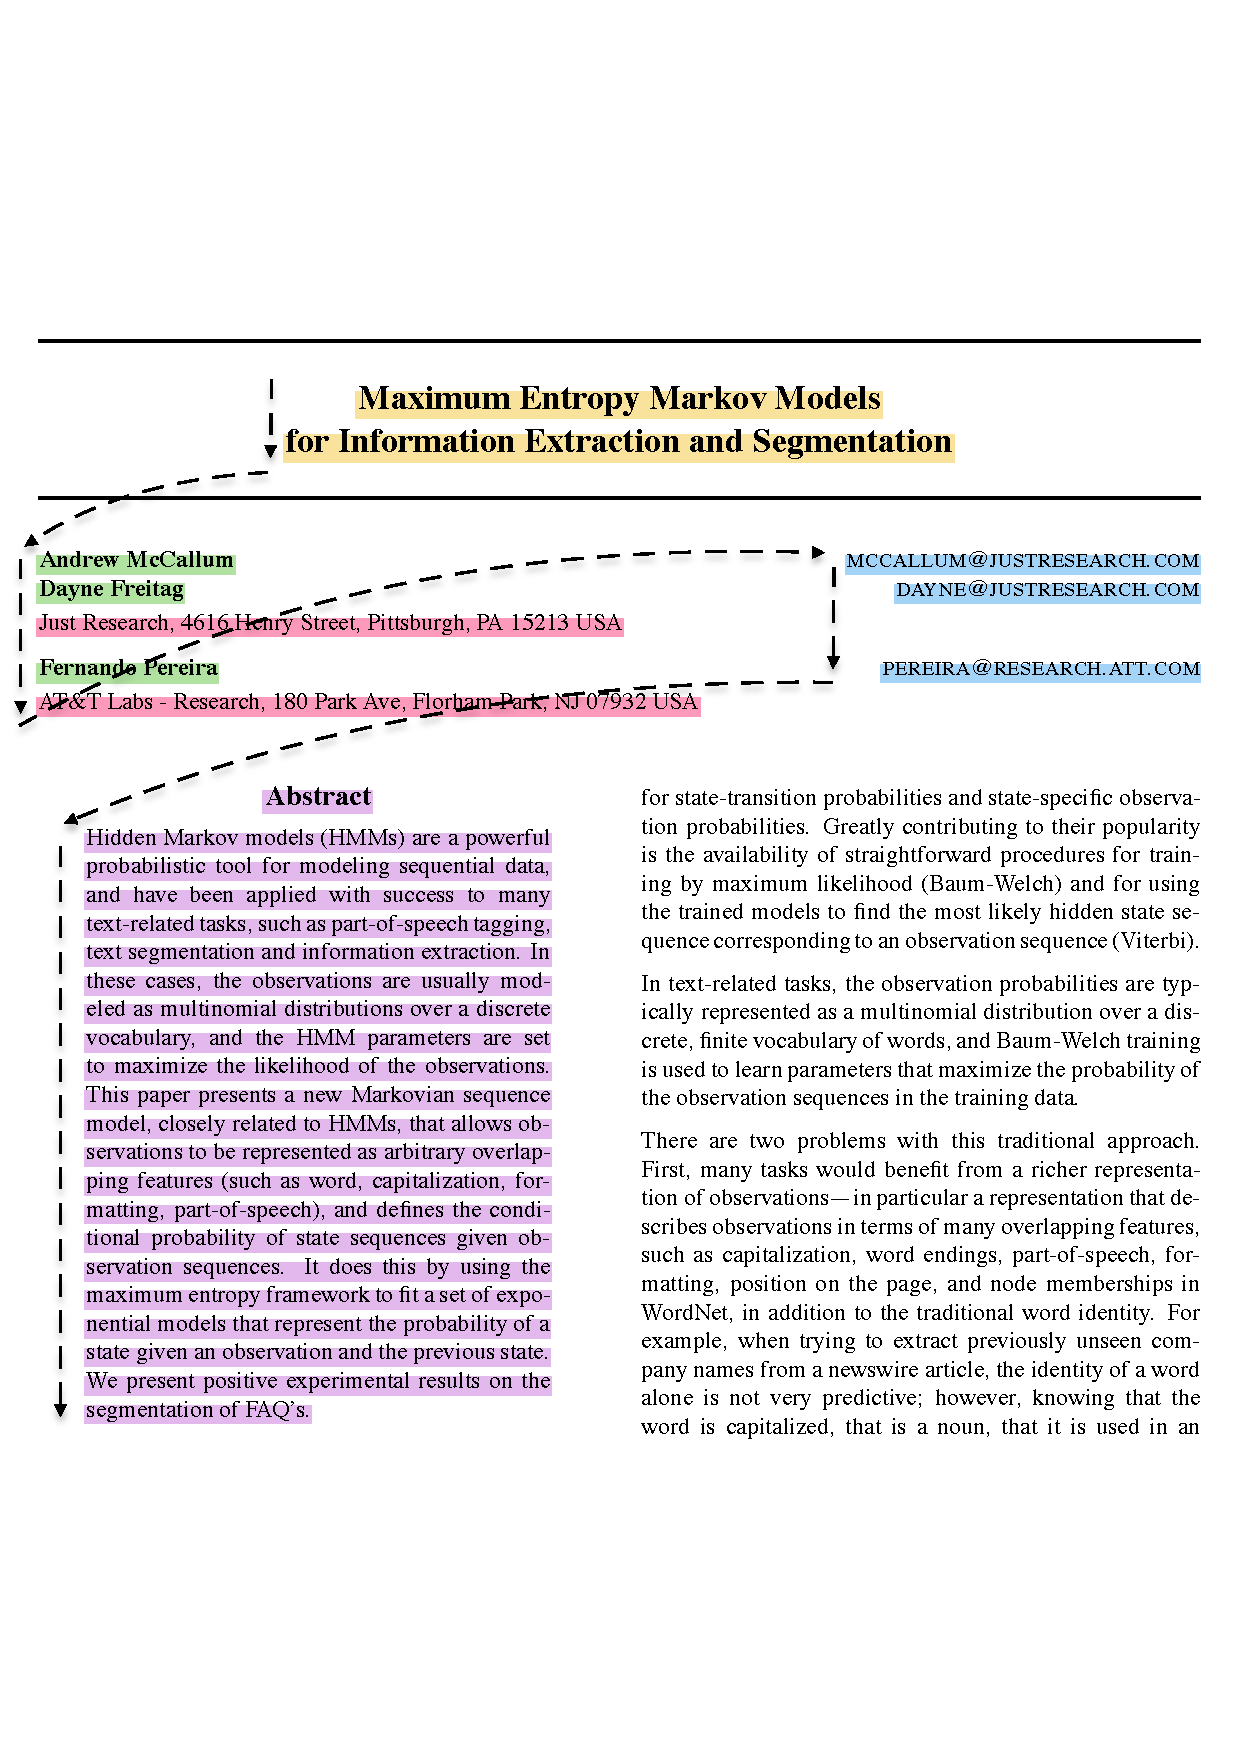
\includegraphics[width=\textwidth]{Figures/extraction.pdf}
\caption{An illustration of the way a header section might be segmented and classified. The classes modelled are colour-coded (title in yellow, authors in green, and so on).}
\label{fig:grobid}
\end{figure}

\section{Solution Methods}

A 2013 study of metadata extraction techniques \cite{lipinski2013evaluation} identified three fundamental methods for AME:

\begin{enumerate}
\item stylistic analysis;
\item knowledge base, and;
\item machine learning approaches.
\end{enumerate}

\emph{Stylistic analysis} refers to heuristic approaches to analysing physical characteristics of text font and layout. \emph{Knowledge base} methods rely on online repositories to cross-reference extracted information. \emph{Machine learning} refers here either to the state-of-the-art conditional random fields, or to other approaches such as hidden Markov models or support vector machines. There is evidence to suggest that the best approach is a combination of the three methods,as software systems such as GROBID (Section \ref{sec:grobid}) do. The study includes a comparison of the leading AME tools based on an \emph{ad hoc} scoring system over fixed header test data. GROBID performed best by a considerable margin, ahead of commercial applications Mendeley Desktop and ParsCit.

\section{GROBID}
\label{sec:grobid}
GROBID (GeneRatiOn of BIbliographic Data) (\cite{lopez2009grobid}) is an open-source (Apache license) Java-based tool for automatic metadata extraction of scientific articles. It has been in development by Patrice Lopez at the French Institute for Research in Computer Science and Automation (INRIA) since 2008. GROBID manages the training, evaluation and application of a hierarchy of Wapiti-trained CRF models, each addressing a part of the information extraction of scientific articles. Figure \ref{fig:cascade} shows the \emph{cascade} of models used to progressively refine classifications of article content. Through GROBID, higher-tier models such as the \emph{header} and \emph{reference} models may be applied individually to PDFs, while the other, more specific models, such as the \emph{date} model, operate only on plaintext inputs. Moreover, some models, such as \emph{segmentation}, are not intended to be used independently, but rather contribute to the cascade, supplying lower levels with their inputs. For example, reference extraction begins with the \emph{segmentation} model, which classifies each line of a document, resulting in homogeneous blocks of lines, for example, header, paragraph, figure, and references. This information is then distributed to the other models, for example the \emph{reference segmenter} model, which further breaks down the reference list into individual references. The \emph{citation} model then classifies the parts of each reference into classes, for example, \emph{date}, \emph{affiliation}, and \emph{author}. Finally, the atomic subcomponents of these are classified by their respective models. Note that the \emph{citation} branch of the cascade has the option of further cross-checking extracted references with the third-party CrossRef web service\footnote{CrossRef is an online DOI agency with a REST API.}. Thus, the overall accuracy of the system is dependent on the combined accuracy of models in the cascade. Conversely, any errors are propagated down the hierarchy. Though they have much in common, the models vary in the classifications they assign, the features they exploit, and, due to the varying size of the vocabulary (compare say, the number of possible month names to the number of possible author names), the size (dimensionality) of the models. Table \ref{table:featurelist} summarises each of GROBID's models. Calling GROBID function \texttt{processFullText} runs all available models on a batch of PDF documents and classifies each document entirely.

\begin{center}
\begin{table}
\begin{tabular}{ | p{0.15\linewidth} | p{0.35\linewidth} | p{0.4\linewidth} |}
    \hline
    Model & Description & Labels \\ \hline
    Header & Classifies front matter & <title>, <author>, <affiliation>, <reference>, <submission>, <abstract>, <address>, <keyword>, <degree>, <pubnum>, <email>, <date>, <copyright>, <intro>, <web>, <note>, <phone>, <dedication>, <entitle>, <grant>, <date-submission> \\ \hline
    Affiliation address & Classifies the components of author affiliations and affiliation addresses. Subordinate to the \emph{header} model. & <institution>, <other>, <settlement>, <department>, <postcode>, <country>, <marker>, <region>, <addrLine>, <laboratory>, <postbox>, <other>, <null> \\ \hline
    Name/ Header & Classifies an author's full name (as identified by the \emph{header} model) into first and last name etc.  & <forename>, <surname>, <marker>, <middlename>, <other>, <suffix>, <title> \\ \hline
    Name/ Citation &  Classifies an author's full name (as identified by the \emph{citation} model) into first and last name etc. & <surname>, <forename>, <other>, <middlename> \\ \hline
    Citation & Classifies a reference into its subcomponents. & <journal>, <volume>, <other>, <issue>, <pages>, <date>, <author>, <title>, <booktitle>, <location>, <pubnum>, <note>, <publisher>, <editor>, <institution>, <tech>, <web>, <issue> \\ \hline
    Date & Classifies the components of a date string identified by higher-tier models. & <other>, <day>, <month>, <year> \\ \hline
    Segmentation & The highest-level model in the architecture--primarily supplies the three models beneath it (header, fulltext and reference-segmenter) with inputs. & <headnote>, <header>, <body>, <page>, <references>, <footnote>, <cover>, <acknowledgement>, <annex> \\ \hline
    Reference-Segmenter & Segments a full reference list into individual citations. & <label>, <reference>, <other> \\ \hline
    Fulltext & Classifies elements of article body. & <section>, <paragraph>, <citation\_marker>, <other>, <table\_marker>, <figure\_marker>, <figure\_head>, <trash>, <figDesc>, <equation>, <item> \\ \hline
\end{tabular}
\caption{A summary of the models coordinated by GROBID. We have here excluded the Patent, Entities, and E-book models as these are experimental models not currently used by GROBID.}
\label{table:featurelist}
\end{table}
\end{center}

\subsection{Text Encoding Initiative}
\label{subsec:tei}
One of GROBID's functions is to transform Wapiti outputs into an output conforming to the Text Encoding Initiative (TEI) standard, therefore we briefly describe it here. TEI is a text encoding standard maintained by the TEI consortium. It specifies an XML representation of a document's contents from the front matter, to the document body, to the document rear. It gives structure and semantic meaning to document components, and can facilitate highly detailed representations. It is therefore apt as a format for annotating a document's metadata. GROBID uses TEI to format its outputs, as well as its training data. In Figure \ref{fig:tei}, we show a sample of a TEI document used to represent a date. The structured XML format can be used to give semantic information about the information enclosed. There is thus a natural mapping between metadata classification and the TEI schema.

\begin{figure}
\lstset{language=XML}
\begin{lstlisting}
<bibl>
    <author>V. Gundelach and D. Eisenburger</author>, &quot; 
    <title level="a">Principle of a direction sensitive borehole antenna with advanced technology and data examples</title>, &quot; in 
    <title level="m">Proceedings of the 4th International Workshop on Advanced Ground Penetrating Radar (IWAGPR &apos;07)</title>, pp. 
    <biblScope type="pp">28-31</biblScope>, 
    <date>June 2007</date>.
</bibl>
\end{lstlisting}
\caption{Sample tagged citation for GROBID training input.}
\label{fig:tei}
\end{figure}

\subsection{Training}
\label{subsec:training}

In GROBID, models are trained in isolation. The models produced by Wapiti (Section \ref{sec:wapiti}) are stored in the GROBID project directory. Each model has its own training data, and feature function templates. For certain models, such as the \emph{header} and \emph{segmentation} models, training data consists of pairs of associated files including:

\begin{enumerate}
\item a TEI file, and;
\item a raw feature file containing extracted features.
\end{enumerate}

Other, simpler models, require only the former. Together, the files form an abstraction over the CRF engine inputs. The reason for including the feature files is because the original PDF files are assumed not to be available at training time, and therefore any features derived from text styling or positioning must be extracted in advance. The TEI files simply provide the classifications of the plaintext required to build a ground truth. The feature extraction itself is done by a module of GROBID. Since feature files and feature template files, which are configured manually by the developer, must agree, there is a strong coupling between this module and the templates.

\subsection{Evaluation}

Both training and evaluation are performed on sets of TEI documents (see Section \ref{subsec:tei} and Figure \ref{fig:tei}). This somewhat paradoxically, when prediction is based on PDF files. However, with closer inspection, an equivalence can be seen between:

\begin{enumerate}
\item applying the \emph{pdftoxml} tool, tokenising the output and transforming to CRF input data, and;
\item extracting tokens from TEI documents (and possibly feature files also--see Section \ref{subsec:training}), and transforming to CRF input data.
\end{enumerate}

Both approaches yield the same input data for the CRF engine, and so the evaluation inputs are, in effect, the same as for prediction, despite the initial differences.

Training may be done with a split defined by the developer, which GROBID uses to set aside a proportion of the training data for evaluation. The evaluation of a model produced by training follows identical procedures, preparing the same input data. The output, however, is not a model but the tagged data. GROBID compares these predictions with the ground truth and reports \emph{accuracy}, \emph{precision}, \emph{recall}, and \emph{F1} scores as performance indicators, at the token, field, and instance levels. A token usually refers to a single contiguous string of characters (without spaces), but in the case of the \emph{segmentation} and \emph{fulltext}, a token is a line. A field is a block of contiguous tokens sharing a class, and an instance is the whole data sample. The accuracy of an instance is therefore judged by the correctness of all tagging for the whole sample (which may a whole document), a difficult thing to achieve without any mistakes.

\subsection{Prediction}

Figure \ref{fig:flow} shows the flow of information from input to output, as well as the relationship between training and prediction. When it comes to labelling (prediction), the starting point is a PDF document. With a third-party tool, \emph{pdftoxml}, this is transformed into an XML file containing rich text information (font, style, orientation) for every string token in the document. This information is stored in \texttt{LayoutToken} objects within GROBID. These tokens are arranged into blocks and features are extracted as they were for training and evaluation. The model created in the training phase is first loaded, and then the \emph{EngineTagger} module calls the CRF engine to label the inputs. Unlike for training, the feature template file is not required, as these have already been absorbed into the model file. After processing, Wapiti returns the same file with classifications inserted. GROBID then further processes this information to transform it into the final TEI output format.

\subsection{Other Functionality}

In addition to the above, GROBID provides a means of producing training sets semi-automatically. This consists of applying the existing models on a batch PDF training set to produce the XML inputs. Of course, each field must be checked against a ground truth and errors corrected before it is used as a training set. We use this functionality to generate training data for benchmarking GROBID on HEP papers (see Chapter \ref{Chapter4}).

\begin{figure}[!ht]
\center
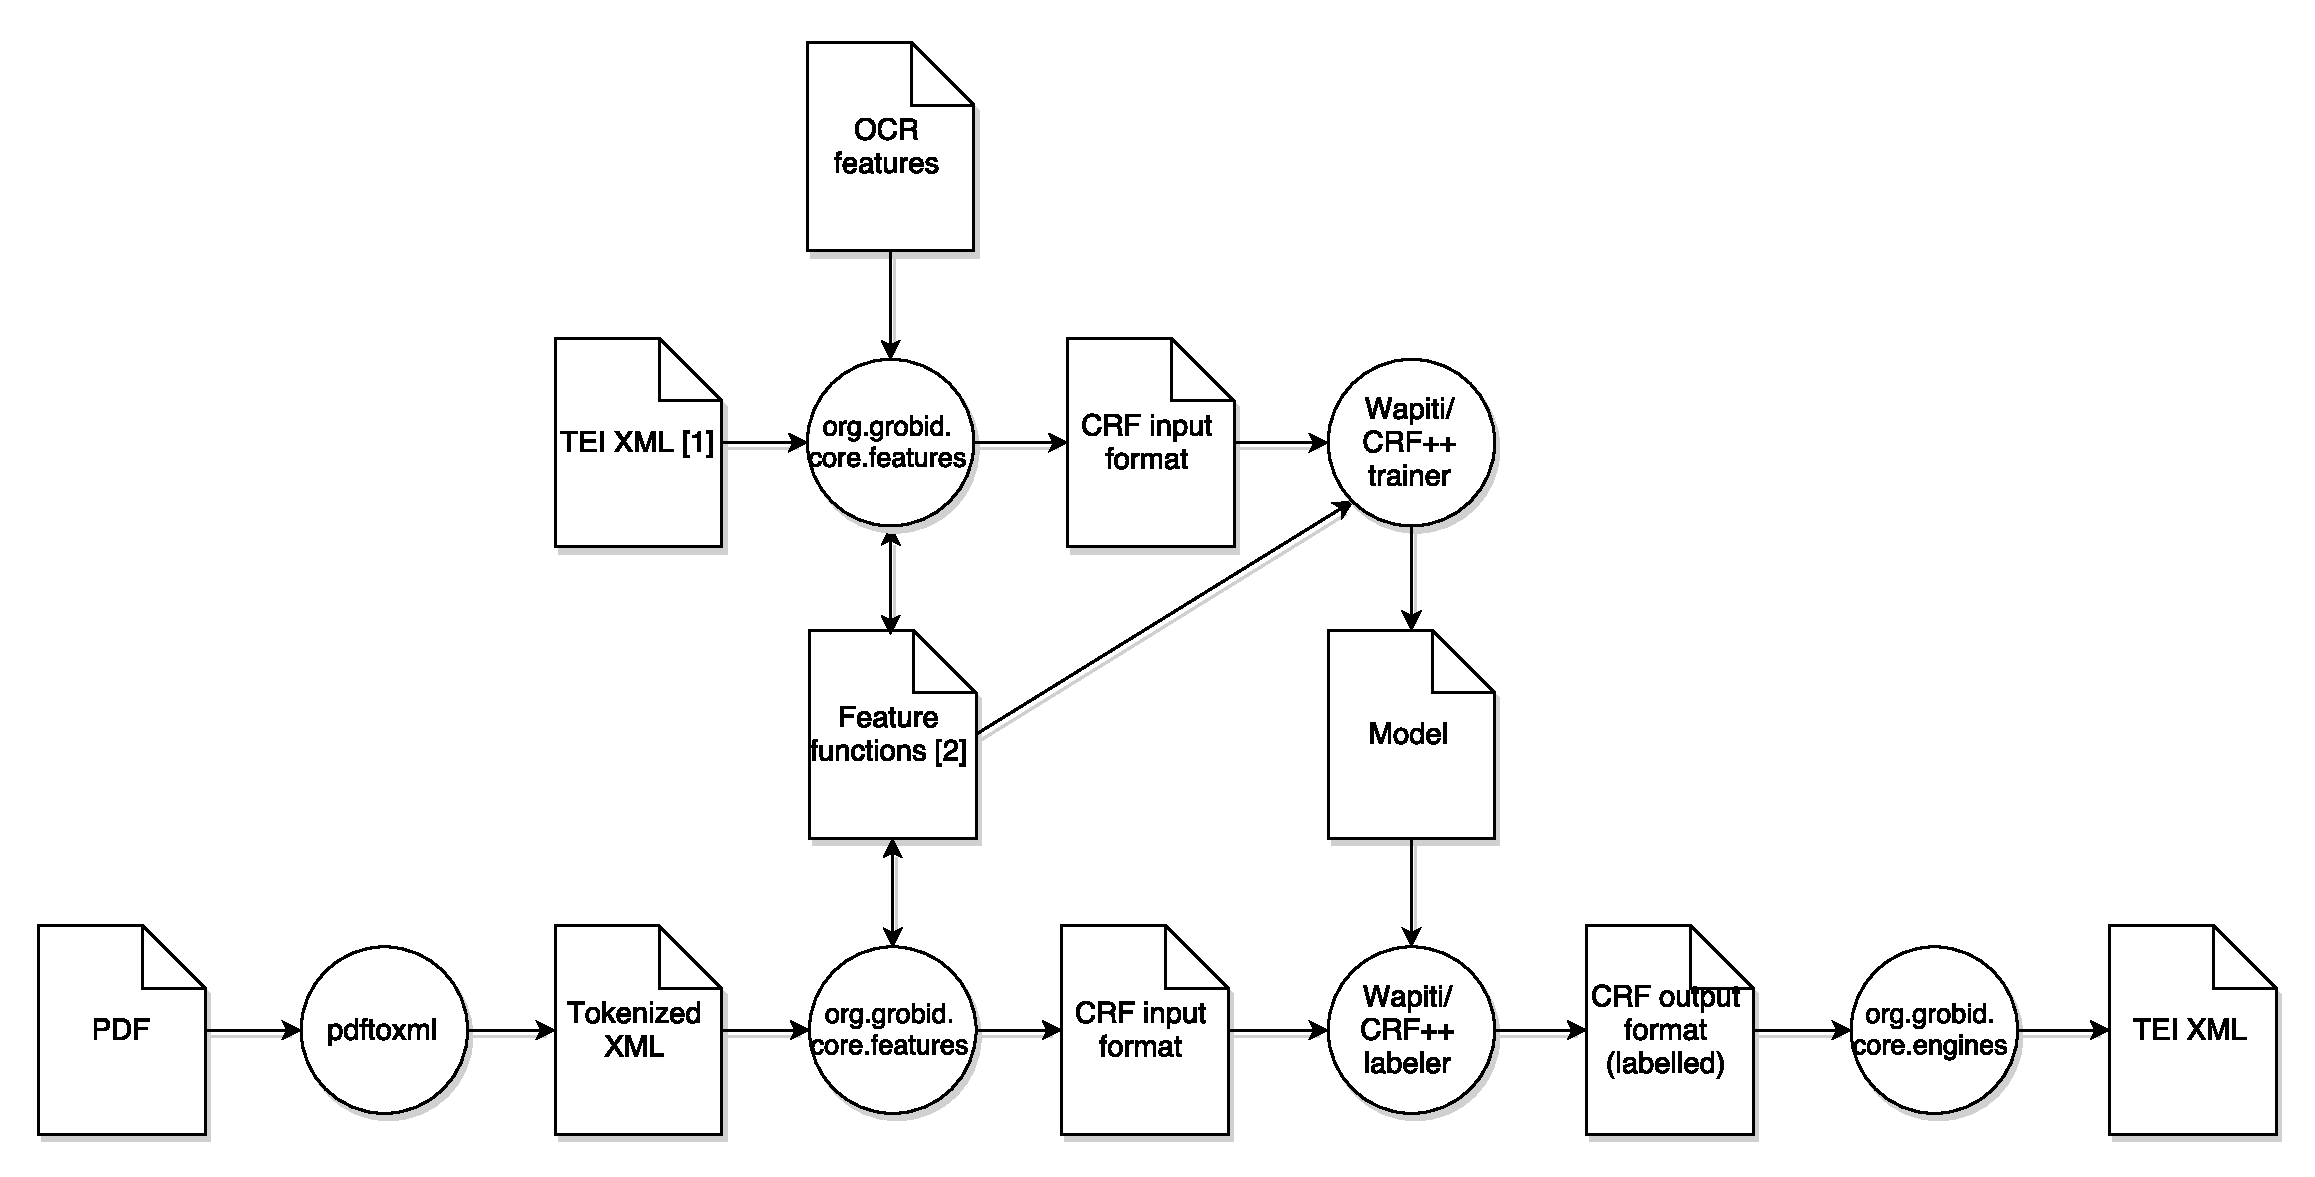
\includegraphics[width=\textwidth]{Figures/grobid.pdf}
\caption{An illustration of the interactions between GROBID and Wapiti for the two main functions of training and tagging. The dashed arrows indicate training operations; the solid arrows, tagging.}
\label{fig:flow}
\end{figure}

\begin{figure}[!ht]
\center
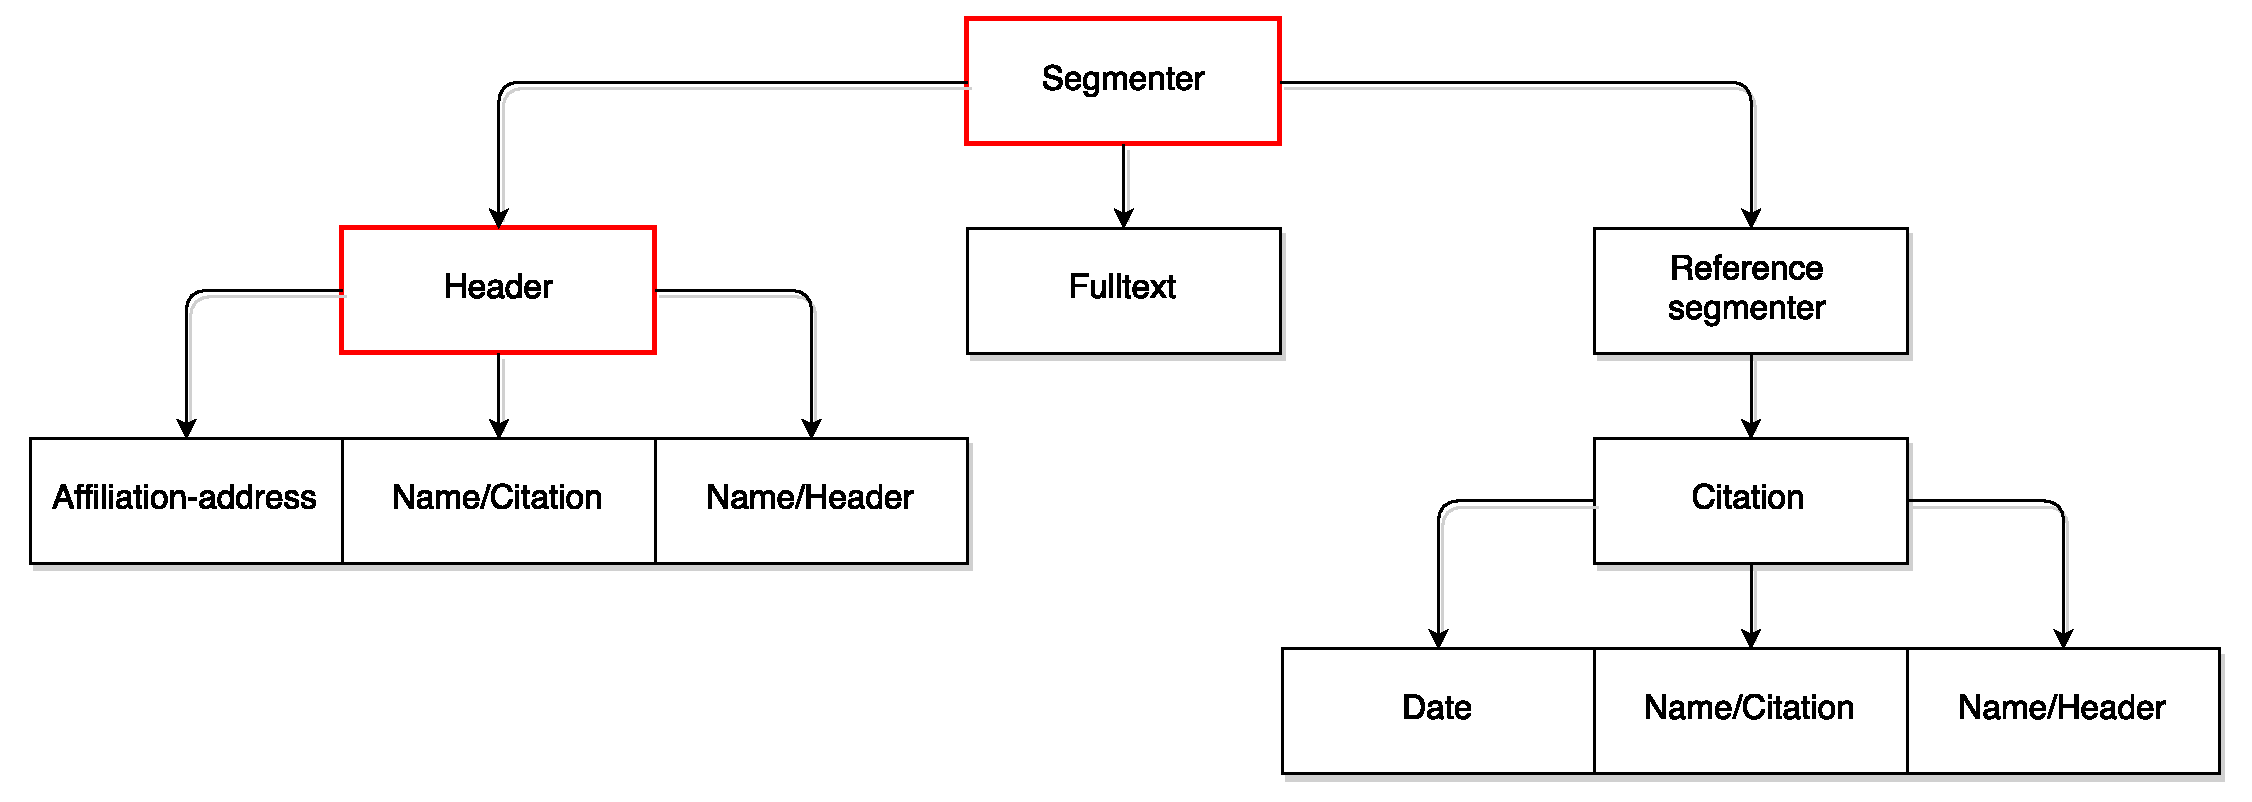
\includegraphics[width=\textwidth]{Figures/cascade.pdf}
\caption{The models of GROBID are organised into a cascade, where each part of a document is classified in increasingly greater detail.}
\label{fig:cascade}
\end{figure}


